\subsubsection{错误概率与功效函数}\label{sec:8.3.1}
检验 $H_0:\theta\in\Theta_0$ 对 $H_1:\theta\in\Theta_0^c$，可能犯两种错误中的一种. 传统上，这两种错误被赋予不易帮助记忆的名称：第一类错误（Type I Error）和第二类错误（Type II Error\mbox{）.} 若 $\theta\in\Theta_0$，检验却错误地决定拒绝 $H_0$，就犯了第一类错误. 反之，若 $\theta\in\Theta_0^c$，检验却决定接受 $H_0$，就犯了第二类错误. \autoref{tab:8.3.1}描述了这两种不同情形.

\begin{table}[htbp]\centering
\caption{假设检验中的两类错误}\label{tab:8.3.1}\index{SI0513@第一类错误}\index{SI0514@第二类错误}
\begin{tabular}{cc|cc}\toprule
&&\multicolumn{2}{c}{决策}\\
&&接受 $H_0$&拒绝 $H_0$\\\midrule
\multirow{2}{*}{真实状态}&$H_0$&正确决策&第一类错误\\
&$H_1$&第二类错误&正确决策\\\bottomrule
\end{tabular}
\end{table}

设 $R$ 表示某检验的拒绝域. 对 $\theta\in\Theta_0$，如果 $\boldsymbol x\in R$，检验就会犯错，故第一类错误的概率为 $P_\theta(\boldsymbol X\in R)$. 对 $\theta\in\Theta_0^c$，第二类错误的概率为 $P_\theta(\boldsymbol X\in R^c)$. 从 $R$ 转到 $R^c$ 略显混乱，但注意到 $P_\theta(\boldsymbol X\in R^c)=1-P_\theta(\boldsymbol X\in R)$，便知 $\theta$ 的函数 $P_\theta(\boldsymbol X\in R)$ 包含了有关拒绝域为 $R$ 的检验的全部信息. 有
$$P_\theta(\boldsymbol X\in R)=\begin{cases}\text{第一类错误的概率},&\theta\in\Theta_0,\\1-\text{第二类错误的概率},&\theta\in\Theta_0^c.\end{cases}$$
这一考虑引出如下定义.
\begin{definition}\label{def:8.3.1}\index{SI0501@功效}
拒绝域为 $R$ 的假设检验的功效函数（power function）是 $\theta$ 的函数 $\beta(\theta)=P_\theta(\boldsymbol X\in R)$.
\end{definition}
理想的功效函数对所有 $\theta\in\Theta_0$ 为零，对所有 $\theta\in\Theta_0^c$ 为一. 除平凡情形外，这一理想无法实现. 定性地说，好的检验应对大多数 $\theta\in\Theta_0^c$ 具有接近一的功效，对大多数 $\theta\in\Theta_0$ 具有接近零的功效.
\begin{example}[二项功效函数]\label{ex:8.3.2}\index{SI0502@二项}
设 $X\sim\operatorname{binomial}(5,\theta)$. 考虑检验 $H_0:\theta\le1/2$ 对 $H_1:\theta>1/2$. 先考虑仅在观察到全部“成功”时才拒绝 $H_0$ 的检验，其功效函数为
$$\beta_1(\theta)=P_\theta(\boldsymbol X\in R)=P_\theta(X=5)=\theta^5.$$
$\beta_1(\theta)$ 的图像见\autoref{fig:8.3.1}. 考察该功效函数，可能认为虽然第一类错误概率低到可以接受（对所有 $\theta\le1/2$，$\beta_1(\theta)\le(1/2)^5=.0312$），但对大多数 $\theta>1/2$，第二类错误概率太高（$\beta_1(\theta)$ 太小\mbox{）.} 只有当 $\theta>(1/2)^{1/5}=.87$ 时，第二类错误概率才小于 $1/2$. 为降低第二类错误概率，可以考虑在 $X=3,4,5$ 时拒绝 $H_0$ 的检验，其功效函数为
$$\begin{aligned}
\beta_2(\theta)&=P_\theta(X=3,4\text{ 或 }5)\\
&=\binom53\theta^3(1-\theta)^2+\binom54\theta^4(1-\theta)^1+\binom55\theta^5(1-\theta)^0.
\end{aligned}$$
\sourcepageanchor{342}

\begin{figure}[htbp]\centering
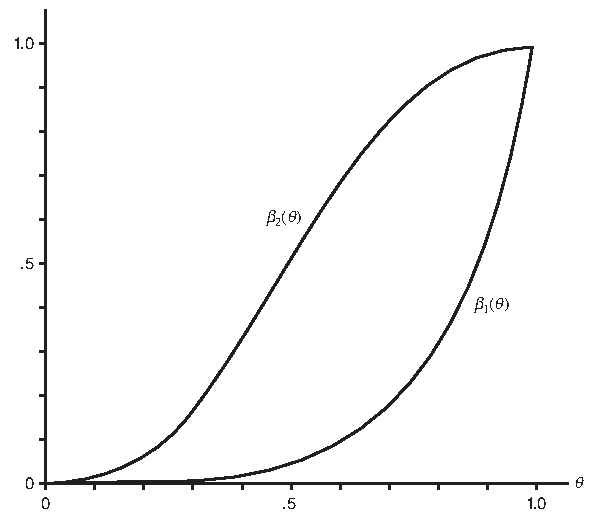
\includegraphics[width=.75\textwidth]{assets/chapter8/fig8-3-1.pdf}
\caption{\autoref{ex:8.3.2}的功效函数.}\label{fig:8.3.1}
\end{figure}

$\beta_2(\theta)$ 也画在\autoref{fig:8.3.1}中. 可见第二个检验确实减小了第二类错误概率，因为对 $\theta>1/2$，$\beta_2(\theta)$ 更大. 但第二个检验的第一类错误概率也更大，因为对 $\theta\le1/2$，$\beta_2(\theta)$ 也更大. 若要在两者之间选择，研究者必须决定哪一种错误结构——由 $\beta_1(\theta)$ 还是由 $\beta_2(\theta)$ 描述的结构——更可接受.
\end{example}
\begin{example}[正态功效函数]\label{ex:8.3.3}\index{SI0504@正态}
设 $X_1,\ldots,X_n$ 是来自 $\mathrm n(\theta,\sigma^2)$ 总体的随机样本，$\sigma^2$ 已知. 检验 $H_0:\theta\le\theta_0$ 对 $H_1:\theta>\theta_0$ 的一种似然比检验，是当 $(\bar X-\theta_0)/(\sigma/\sqrt n)>c$ 时拒绝 $H_0$（\autoref{exercise:8.37}\mbox{）.} 常数 $c$ 可以是任意正数. 其功效函数为
$$\begin{aligned}
\beta(\theta)&=P_\theta\left(\frac{\bar X-\theta_0}{\sigma/\sqrt n}>c\right)\\
&=P_\theta\left(\frac{\bar X-\theta}{\sigma/\sqrt n}>c+\frac{\theta_0-\theta}{\sigma/\sqrt n}\right)\\
&=P\left(Z>c+\frac{\theta_0-\theta}{\sigma/\sqrt n}\right),
\end{aligned}$$
其中 $Z$ 为标准正态随机变量，因为 $(\bar X-\theta)/(\sigma/\sqrt n)\sim\mathrm n(0,1)$. 容易看出，当 $\theta$ 从 $-\infty$ 增至 $\infty$ 时，这一正态概率从零增至一. 因此 $\beta(\theta)$ 是 $\theta$ 的增函数，并且
$$\lim_{\theta\to-\infty}\beta(\theta)=0,\qquad\lim_{\theta\to\infty}\beta(\theta)=1,\qquad
\beta(\theta_0)=\alpha\ \text{若 }P(Z>c)=\alpha.$$
\autoref{fig:8.3.2}给出了 $c=1.28$ 时的 $\beta(\theta)$ 图像.
\end{example}
通常，检验的功效函数依赖样本量 $n$. 若 $n$ 可由实验者选择，考虑功效函数就可能帮助确定实验中适当的样本量.
\sourcepageanchor{343}

\begin{figure}[htbp]\centering
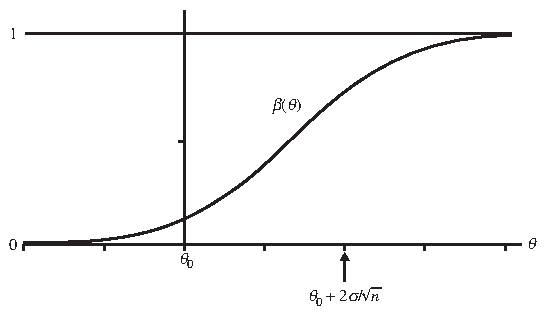
\includegraphics[width=.78\textwidth]{assets/chapter8/fig8-3-2.pdf}
\caption{\autoref{ex:8.3.3}的功效函数.}\label{fig:8.3.2}
\end{figure}

\begin{example}[续\autoref{ex:8.3.3}]\label{ex:8.3.4}\index{SI0510@正态}\index{SI0513@第一类错误}\index{SI0514@第二类错误}\index{SI0947@假设检验：正态}
假设实验者希望最大第一类错误概率为 $.1$；此外，希望在 $\theta\ge\theta_0+\sigma$ 时，最大第二类错误概率为 $.2$. 现在说明如何选择 $c$ 和 $n$ 达到这些目标，采用的检验是在 $(\bar X-\theta_0)/(\sigma/\sqrt n)>c$ 时拒绝 $H_0:\theta\le\theta_0$. 如上所述，这种检验的功效函数为
$$\beta(\theta)=P\left(Z>c+\frac{\theta_0-\theta}{\sigma/\sqrt n}\right).$$
由于 $\beta(\theta)$ 随 $\theta$ 递增，只要
$$\beta(\theta_0)=.1\quad\text{且}\quad\beta(\theta_0+\sigma)=.8,$$
就满足要求.

选择 $c=1.28$，无论 $n$ 为何，都有 $\beta(\theta_0)=P(Z>1.28)=.1$. 现在要选取 $n$，使 $\beta(\theta_0+\sigma)=P(Z>1.28-\sqrt n)=.8$. 因 $P(Z>-.84)=.8$，令 $1.28-\sqrt n=-.84$，解得 $n=4.49$. 当然，$n$ 必须是整数，所以取 $c=1.28$、$n=5$，即可按实验者的规定控制错误概率.\footnote{译注：这里的正态分位数和概率均经过舍入，原文用等号表示近似值. 实际上 $P(Z>1.28)\approx.10027$，略大于 $.1$；若要求严格不超过 $.1$，应取 $c=z_{.1}\approx1.28155$，此时取 $n=5$ 仍满足第二类错误的要求.}
\end{example}
样本量固定时，通常不可能把两类错误概率都任意缩小. 寻找好的检验时，通常先把考虑范围限制为能将第一类错误概率控制在指定水平的检验，再在这一类中寻找第二类错误概率尽可能小的检验. 讨论第一类错误概率的控制时，下列两个术语很有用.
\begin{definition}\label{def:8.3.5}\index{SI0511@检验大小}
对 $0\le\alpha\le1$，若功效函数为 $\beta(\theta)$ 的检验满足 $\sup_{\theta\in\Theta_0}\beta(\theta)=\alpha$，则称其为大小为 $\alpha$ 的检验（size $\alpha$ test\mbox{）.}
\end{definition}
\begin{definition}\label{def:8.3.6}\index{SI0498@检验水平}
对 $0\le\alpha\le1$，若功效函数为 $\beta(\theta)$ 的检验满足 $\sup_{\theta\in\Theta_0}\beta(\theta)\le\alpha$，则称其为水平为 $\alpha$ 的检验（level $\alpha$ test\mbox{）.}
\end{definition}
有些作者不像我们这样区分大小（size）与水平（level），有时两词互换使用. 但按本书的定义，水平为 $\alpha$ 的检验集合包含大小为 $\alpha$ 的检验集合. 而且，在复杂模型和复杂检验问题中，这一区别很重要，因为计算上往往无法构造大小恰为 $\alpha$ 的检验. 此时实验者必须满足于水平为 $\alpha$ 的检验，意识到可能需要某些折中.
\sourcepageanchor{344}
后面会看到一些例子，特别是在并交检验和交并检验中.

实验者通常指定所用检验的水平，典型选择为 $\alpha=.01,.05,.10$. 要注意，固定检验水平只控制第一类错误概率，并不控制第二类错误. 采用这种方法时，应恰当设置原假设和备择假设，使控制第一类错误概率成为最重要的事情. 例如，某实验者期待实验支持一个特定假设，但除非数据确实给出令人信服的支持，否则不愿作出断言. 可以把检验设置成：备择假设正是她期待数据支持、希望证明的假设. （在这一语境下，备择假设有时称为研究假设（research hypothesis\mbox{）.}\index{SI0479@研究}\semanticindexanchor{479:344}）通过采用 $\alpha$ 较小的水平 $\alpha$ 检验，她就能防范在研究假设为假时声称数据支持它.

\autoref{sec:8.2}的方法通常给出检验统计量和拒绝域的一般形式，却通常不会确定某一个具体检验. 例如，似然比检验（\autoref{def:8.2.1}）在 $\lambda(\boldsymbol X)\le c$ 时拒绝 $H_0$，但 $c$ 未指定，所以定义的是整类似然比检验，每个 $c$ 值对应一个. 现在将范围限制为大小 $\alpha$ 的检验，就可能从中选出一个.
\begin{example}[似然比检验的大小]\label{ex:8.3.7}\index{SI0634@指数}\index{SI0638@正态}
一般地，选择 $c$ 使 $\sup_{\theta\in\Theta_0}P_\theta(\lambda(\boldsymbol X)\le c)=\alpha$，便构造出大小为 $\alpha$ 的似然比检验. 如何确定 $c$，依具体问题而定. 例如，在\autoref{ex:8.2.2}中，$\Theta_0$ 只含单点 $\theta=\theta_0$，且在此点 $\sqrt n(\bar X-\theta_0)\sim\mathrm n(0,1)$. 因而，检验
$$\text{若 }|\bar X-\theta_0|\ge z_{\alpha/2}/\sqrt n,\quad\text{则拒绝 }H_0,$$
就是大小为 $\alpha$ 的似然比检验；其中 $z_{\alpha/2}$ 满足 $P(Z\ge z_{\alpha/2})=\alpha/2$，$Z\sim\mathrm n(0,1)$. 具体而言，这相当于取 $c=\exp(-z_{\alpha/2}^2/2)$，但这一点并不重要.

对\autoref{ex:8.2.3}的问题，原假设 $H_0:\theta\le\theta_0$ 包含不止一个点，因此寻找大小为 $\alpha$ 的似然比检验更加复杂. 检验在 $X_{(1)}\ge c$ 时拒绝 $H_0$，其中 $c$ 应使检验大小为 $\alpha$. 但若 $c=(-\log\alpha)/n+\theta_0$，则
$$P_{\theta_0}(X_{(1)}\ge c)=e^{-n(c-\theta_0)}=\alpha.$$
由于 $\theta$ 是 $X_{(1)}$ 的位置参数，
$$P_\theta(X_{(1)}\ge c)\le P_{\theta_0}(X_{(1)}\ge c),\qquad\text{对任意 }\theta\le\theta_0.$$
因此，
$$\sup_{\theta\in\Theta_0}\beta(\theta)=\sup_{\theta\le\theta_0}P_\theta(X_{(1)}\ge c)
=P_{\theta_0}(X_{(1)}\ge c)=\alpha,$$
这个 $c$ 就给出了大小为 $\alpha$ 的似然比检验.
\end{example}
\emph{记号说明：}上例用 $z_{\alpha/2}$ 表示标准正态密度曲线下右侧概率为 $\alpha/2$ 的点. 我们将普遍使用这种记法，不仅用于正态分布，也用于其他分布（为清楚起见，会按需给出定义\mbox{）.} 例如，$z_\alpha$ 满足 $P(Z>z_\alpha)=\alpha$，其中 $Z\sim\mathrm n(0,1)$；$t_{n-1,\alpha/2}$ 满足 $P(T_{n-1}>t_{n-1,\alpha/2})=\alpha/2$，其中 $T_{n-1}\sim t_{n-1}$；$\chi^2_{p,1-\alpha}$ 满足 $P(\chi_p^2>\chi^2_{p,1-\alpha})=1-\alpha$，其中 $\chi_p^2$ 是自由度为 $p$ 的卡方随机变量. $z_{\alpha/2},z_\alpha,t_{n-1,\alpha/2},\chi^2_{p,1-\alpha}$ 等点称为临界点（cutoff points\mbox{）.}\index{SI0243@临界点}\semanticindexanchor{243:344}
\begin{example}[并交检验的大小]\label{ex:8.3.8}\index{SI0525@正态}\index{SI1028@并交}
在\autoref{ex:8.2.8}中，寻找大小为 $\alpha$ 的并交检验，就是寻找常数 $t_L,t_U$，使
$$\sup_{\theta\in\Theta_0}P_\theta\left(\frac{\bar X-\mu_0}{\sqrt{S^2/n}}\ge t_L\quad\text{或}\quad\frac{\bar X-\mu_0}{\sqrt{S^2/n}}\le t_U\right)=\alpha.$$
\sourcepageanchor{345}
但对任意 $(\mu,\sigma^2)=\theta\in\Theta_0$，都有 $\mu=\mu_0$，因此 $(\bar X-\mu_0)/\sqrt{S^2/n}$ 服从自由度为 $n-1$ 的 Student $t$ 分布. 所以，只要取 $t_U=t_{n-1,1-\alpha_1}$、$t_L=t_{n-1,\alpha_2}$，其中 $\alpha_1+\alpha_2=\alpha$，就得到对所有 $\theta\in\Theta_0$ 第一类错误概率均恰为 $\alpha$ 的检验. 通常取 $t_L=-t_U=t_{n-1,\alpha/2}$.
\end{example}
除了 $\alpha$ 水平，还可能关心检验的其他特征. 例如，希望在 $\theta\in\Theta_0^c$ 时，比在 $\theta\in\Theta_0$ 时更可能拒绝 $H_0$. \autoref{fig:8.3.1}和\autoref{fig:8.3.2}的全部功效函数都有此性质，得到的检验称为无偏检验.
\begin{definition}\label{def:8.3.9}\index{SI0520@无偏}
若对每个 $\theta'\in\Theta_0^c$ 和 $\theta''\in\Theta_0$，都有 $\beta(\theta')\ge\beta(\theta'')$，则功效函数为 $\beta(\theta)$ 的检验称为无偏的（unbiased\mbox{）.}
\end{definition}
\begin{example}[\autoref{ex:8.3.3}的结论]\label{ex:8.3.10}
检验 $H_0:\theta\le\theta_0$ 对 $H_1:\theta>\theta_0$ 的似然比检验具有功效函数
$$\beta(\theta)=P\left(Z>c+\frac{\theta_0-\theta}{\sigma/\sqrt n}\right),$$
其中 $Z\sim\mathrm n(0,1)$. 由于对固定 $\theta_0$，$\beta(\theta)$ 是 $\theta$ 的增函数，故
$$\beta(\theta)>\beta(\theta_0)=\max_{t\le\theta_0}\beta(t),\qquad\text{对所有 }\theta>\theta_0,$$
所以该检验无偏.
\end{example}
多数问题有许多无偏检验（见\autoref{exercise:8.45}\mbox{）.} 同样，大小为 $\alpha$ 的检验、似然比检验等也往往有许多个. 有时施加的限制已足以把考虑范围缩减为一个检验. \autoref{ex:8.3.7}中的两个问题，都只有一个大小为 $\alpha$ 的似然比检验. 在其他情形下，仍有许多检验可选；我们只讨论了在 $T$ 较大时拒绝 $H_0$ 的那一个. 接下来将讨论从一类检验中作选择的其他准则，它们都与检验的功效函数有关.
